% Created by tikzDevice version 0.10.1 on 2018-01-15 21:00:09
% !TEX encoding = UTF-8 Unicode
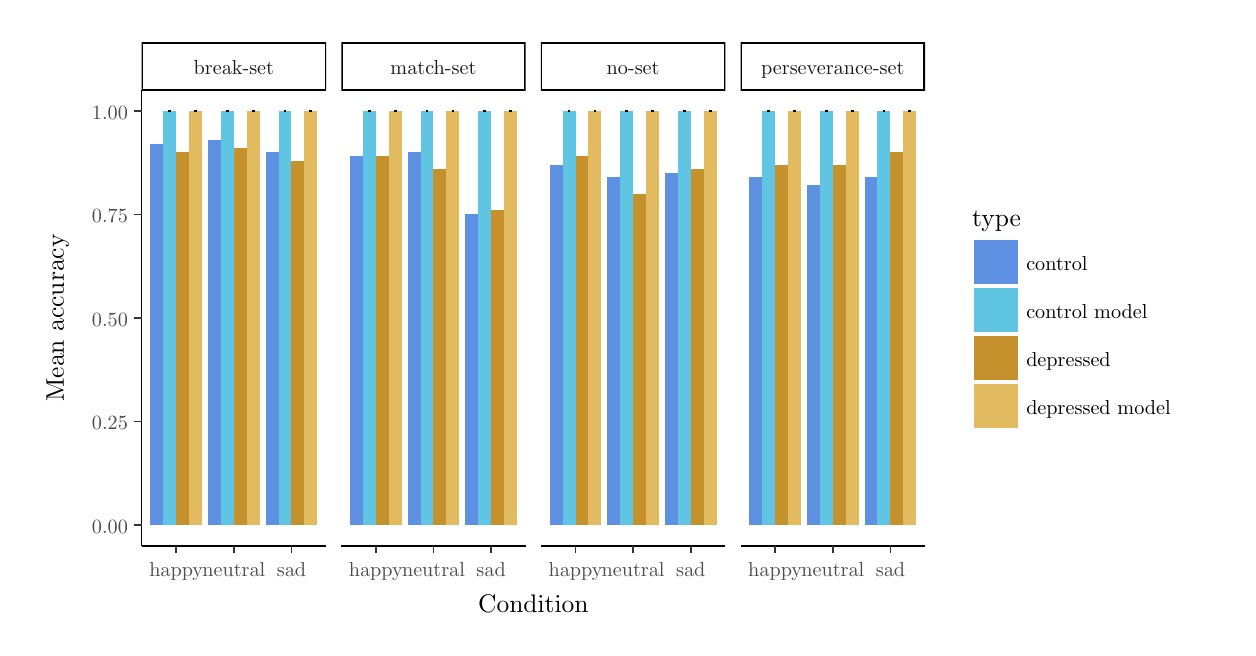
\begin{tikzpicture}[x=1pt,y=1pt]
\definecolor{fillColor}{RGB}{255,255,255}
\path[use as bounding box,fill=fillColor,fill opacity=0.00] (0,0) rectangle (433.62,216.81);
\begin{scope}
\path[clip] (  0.00,  0.00) rectangle (433.62,216.81);
\definecolor{drawColor}{RGB}{255,255,255}
\definecolor{fillColor}{RGB}{255,255,255}

\path[draw=drawColor,line width= 0.6pt,line join=round,line cap=round,fill=fillColor] (  0.00,  0.00) rectangle (433.62,216.81);
\end{scope}
\begin{scope}
\path[clip] ( 41.17, 29.59) rectangle (107.82,194.25);
\definecolor{fillColor}{RGB}{255,255,255}

\path[fill=fillColor] ( 41.17, 29.59) rectangle (107.82,194.25);
\definecolor{fillColor}{RGB}{226,186,95}

\path[fill=fillColor] ( 58.36, 37.07) rectangle ( 63.04,186.76);
\definecolor{fillColor}{RGB}{196,145,45}

\path[fill=fillColor] ( 53.67, 37.07) rectangle ( 58.36,171.80);
\definecolor{fillColor}{RGB}{95,197,226}

\path[fill=fillColor] ( 48.98, 37.07) rectangle ( 53.67,186.76);
\definecolor{fillColor}{RGB}{95,145,226}

\path[fill=fillColor] ( 44.30, 37.07) rectangle ( 48.98,174.79);
\definecolor{fillColor}{RGB}{226,186,95}

\path[fill=fillColor] ( 79.18, 37.07) rectangle ( 83.87,186.76);
\definecolor{fillColor}{RGB}{196,145,45}

\path[fill=fillColor] ( 74.50, 37.07) rectangle ( 79.18,173.29);
\definecolor{fillColor}{RGB}{95,197,226}

\path[fill=fillColor] ( 69.81, 37.07) rectangle ( 74.50,186.76);
\definecolor{fillColor}{RGB}{95,145,226}

\path[fill=fillColor] ( 65.12, 37.07) rectangle ( 69.81,176.29);
\definecolor{fillColor}{RGB}{226,186,95}

\path[fill=fillColor] (100.01, 37.07) rectangle (104.69,186.76);
\definecolor{fillColor}{RGB}{196,145,45}

\path[fill=fillColor] ( 95.32, 37.07) rectangle (100.01,168.80);
\definecolor{fillColor}{RGB}{95,197,226}

\path[fill=fillColor] ( 90.64, 37.07) rectangle ( 95.32,186.76);
\definecolor{fillColor}{RGB}{95,145,226}

\path[fill=fillColor] ( 85.95, 37.07) rectangle ( 90.64,171.80);
\definecolor{drawColor}{RGB}{0,0,0}

\path[draw=drawColor,line width= 0.6pt,line join=round] ( 60.18,186.76) --
	( 61.22,186.76);

\path[draw=drawColor,line width= 0.6pt,line join=round] ( 60.70,186.76) --
	( 60.70,186.76);

\path[draw=drawColor,line width= 0.6pt,line join=round] ( 60.18,186.76) --
	( 61.22,186.76);

\path[draw=drawColor,line width= 0.6pt,line join=round] ( 50.81,186.76) --
	( 51.85,186.76);

\path[draw=drawColor,line width= 0.6pt,line join=round] ( 51.33,186.76) --
	( 51.33,186.76);

\path[draw=drawColor,line width= 0.6pt,line join=round] ( 50.81,186.76) --
	( 51.85,186.76);

\path[draw=drawColor,line width= 0.6pt,line join=round] ( 81.00,186.76) --
	( 82.05,186.76);

\path[draw=drawColor,line width= 0.6pt,line join=round] ( 81.52,186.76) --
	( 81.52,186.76);

\path[draw=drawColor,line width= 0.6pt,line join=round] ( 81.00,186.76) --
	( 82.05,186.76);

\path[draw=drawColor,line width= 0.6pt,line join=round] ( 71.63,186.76) --
	( 72.67,186.76);

\path[draw=drawColor,line width= 0.6pt,line join=round] ( 72.15,186.76) --
	( 72.15,186.76);

\path[draw=drawColor,line width= 0.6pt,line join=round] ( 71.63,186.76) --
	( 72.67,186.76);

\path[draw=drawColor,line width= 0.6pt,line join=round] (101.83,186.76) --
	(102.87,186.76);

\path[draw=drawColor,line width= 0.6pt,line join=round] (102.35,186.76) --
	(102.35,186.76);

\path[draw=drawColor,line width= 0.6pt,line join=round] (101.83,186.76) --
	(102.87,186.76);

\path[draw=drawColor,line width= 0.6pt,line join=round] ( 92.46,186.76) --
	( 93.50,186.76);

\path[draw=drawColor,line width= 0.6pt,line join=round] ( 92.98,186.76) --
	( 92.98,186.76);

\path[draw=drawColor,line width= 0.6pt,line join=round] ( 92.46,186.76) --
	( 93.50,186.76);
\end{scope}
\begin{scope}
\path[clip] (113.32, 29.59) rectangle (179.96,194.25);
\definecolor{fillColor}{RGB}{255,255,255}

\path[fill=fillColor] (113.32, 29.59) rectangle (179.96,194.25);
\definecolor{fillColor}{RGB}{226,186,95}

\path[fill=fillColor] (130.50, 37.07) rectangle (135.19,186.76);
\definecolor{fillColor}{RGB}{196,145,45}

\path[fill=fillColor] (125.81, 37.07) rectangle (130.50,170.30);
\definecolor{fillColor}{RGB}{95,197,226}

\path[fill=fillColor] (121.13, 37.07) rectangle (125.81,186.76);
\definecolor{fillColor}{RGB}{95,145,226}

\path[fill=fillColor] (116.44, 37.07) rectangle (121.13,170.30);
\definecolor{fillColor}{RGB}{226,186,95}

\path[fill=fillColor] (151.33, 37.07) rectangle (156.01,186.76);
\definecolor{fillColor}{RGB}{196,145,45}

\path[fill=fillColor] (146.64, 37.07) rectangle (151.33,165.81);
\definecolor{fillColor}{RGB}{95,197,226}

\path[fill=fillColor] (141.95, 37.07) rectangle (146.64,186.76);
\definecolor{fillColor}{RGB}{95,145,226}

\path[fill=fillColor] (137.27, 37.07) rectangle (141.95,171.80);
\definecolor{fillColor}{RGB}{226,186,95}

\path[fill=fillColor] (172.15, 37.07) rectangle (176.84,186.76);
\definecolor{fillColor}{RGB}{196,145,45}

\path[fill=fillColor] (167.47, 37.07) rectangle (172.15,150.84);
\definecolor{fillColor}{RGB}{95,197,226}

\path[fill=fillColor] (162.78, 37.07) rectangle (167.47,186.76);
\definecolor{fillColor}{RGB}{95,145,226}

\path[fill=fillColor] (158.10, 37.07) rectangle (162.78,149.34);
\definecolor{drawColor}{RGB}{0,0,0}

\path[draw=drawColor,line width= 0.6pt,line join=round] (132.32,186.76) --
	(133.36,186.76);

\path[draw=drawColor,line width= 0.6pt,line join=round] (132.84,186.76) --
	(132.84,186.76);

\path[draw=drawColor,line width= 0.6pt,line join=round] (132.32,186.76) --
	(133.36,186.76);

\path[draw=drawColor,line width= 0.6pt,line join=round] (122.95,186.76) --
	(123.99,186.76);

\path[draw=drawColor,line width= 0.6pt,line join=round] (123.47,186.76) --
	(123.47,186.76);

\path[draw=drawColor,line width= 0.6pt,line join=round] (122.95,186.76) --
	(123.99,186.76);

\path[draw=drawColor,line width= 0.6pt,line join=round] (153.15,186.76) --
	(154.19,186.76);

\path[draw=drawColor,line width= 0.6pt,line join=round] (153.67,186.76) --
	(153.67,186.76);

\path[draw=drawColor,line width= 0.6pt,line join=round] (153.15,186.76) --
	(154.19,186.76);

\path[draw=drawColor,line width= 0.6pt,line join=round] (143.78,186.76) --
	(144.82,186.76);

\path[draw=drawColor,line width= 0.6pt,line join=round] (144.30,186.76) --
	(144.30,186.76);

\path[draw=drawColor,line width= 0.6pt,line join=round] (143.78,186.76) --
	(144.82,186.76);

\path[draw=drawColor,line width= 0.6pt,line join=round] (173.98,186.76) --
	(175.02,186.76);

\path[draw=drawColor,line width= 0.6pt,line join=round] (174.50,186.76) --
	(174.50,186.76);

\path[draw=drawColor,line width= 0.6pt,line join=round] (173.98,186.76) --
	(175.02,186.76);

\path[draw=drawColor,line width= 0.6pt,line join=round] (164.60,186.76) --
	(165.64,186.76);

\path[draw=drawColor,line width= 0.6pt,line join=round] (165.12,186.76) --
	(165.12,186.76);

\path[draw=drawColor,line width= 0.6pt,line join=round] (164.60,186.76) --
	(165.64,186.76);
\end{scope}
\begin{scope}
\path[clip] (185.46, 29.59) rectangle (252.11,194.25);
\definecolor{fillColor}{RGB}{255,255,255}

\path[fill=fillColor] (185.46, 29.59) rectangle (252.11,194.25);
\definecolor{fillColor}{RGB}{226,186,95}

\path[fill=fillColor] (202.64, 37.07) rectangle (207.33,186.76);
\definecolor{fillColor}{RGB}{196,145,45}

\path[fill=fillColor] (197.96, 37.07) rectangle (202.64,170.30);
\definecolor{fillColor}{RGB}{95,197,226}

\path[fill=fillColor] (193.27, 37.07) rectangle (197.96,186.76);
\definecolor{fillColor}{RGB}{95,145,226}

\path[fill=fillColor] (188.59, 37.07) rectangle (193.27,167.30);
\definecolor{fillColor}{RGB}{226,186,95}

\path[fill=fillColor] (223.47, 37.07) rectangle (228.16,186.76);
\definecolor{fillColor}{RGB}{196,145,45}

\path[fill=fillColor] (218.79, 37.07) rectangle (223.47,156.83);
\definecolor{fillColor}{RGB}{95,197,226}

\path[fill=fillColor] (214.10, 37.07) rectangle (218.79,186.76);
\definecolor{fillColor}{RGB}{95,145,226}

\path[fill=fillColor] (209.41, 37.07) rectangle (214.10,162.81);
\definecolor{fillColor}{RGB}{226,186,95}

\path[fill=fillColor] (244.30, 37.07) rectangle (248.98,186.76);
\definecolor{fillColor}{RGB}{196,145,45}

\path[fill=fillColor] (239.61, 37.07) rectangle (244.30,165.81);
\definecolor{fillColor}{RGB}{95,197,226}

\path[fill=fillColor] (234.93, 37.07) rectangle (239.61,186.76);
\definecolor{fillColor}{RGB}{95,145,226}

\path[fill=fillColor] (230.24, 37.07) rectangle (234.93,164.31);
\definecolor{drawColor}{RGB}{0,0,0}

\path[draw=drawColor,line width= 0.6pt,line join=round] (204.47,186.76) --
	(205.51,186.76);

\path[draw=drawColor,line width= 0.6pt,line join=round] (204.99,186.76) --
	(204.99,186.76);

\path[draw=drawColor,line width= 0.6pt,line join=round] (204.47,186.76) --
	(205.51,186.76);

\path[draw=drawColor,line width= 0.6pt,line join=round] (195.10,186.76) --
	(196.14,186.76);

\path[draw=drawColor,line width= 0.6pt,line join=round] (195.62,186.76) --
	(195.62,186.76);

\path[draw=drawColor,line width= 0.6pt,line join=round] (195.10,186.76) --
	(196.14,186.76);

\path[draw=drawColor,line width= 0.6pt,line join=round] (225.29,186.76) --
	(226.34,186.76);

\path[draw=drawColor,line width= 0.6pt,line join=round] (225.81,186.76) --
	(225.81,186.76);

\path[draw=drawColor,line width= 0.6pt,line join=round] (225.29,186.76) --
	(226.34,186.76);

\path[draw=drawColor,line width= 0.6pt,line join=round] (215.92,186.76) --
	(216.96,186.76);

\path[draw=drawColor,line width= 0.6pt,line join=round] (216.44,186.76) --
	(216.44,186.76);

\path[draw=drawColor,line width= 0.6pt,line join=round] (215.92,186.76) --
	(216.96,186.76);

\path[draw=drawColor,line width= 0.6pt,line join=round] (246.12,186.76) --
	(247.16,186.76);

\path[draw=drawColor,line width= 0.6pt,line join=round] (246.64,186.76) --
	(246.64,186.76);

\path[draw=drawColor,line width= 0.6pt,line join=round] (246.12,186.76) --
	(247.16,186.76);

\path[draw=drawColor,line width= 0.6pt,line join=round] (236.75,186.76) --
	(237.79,186.76);

\path[draw=drawColor,line width= 0.6pt,line join=round] (237.27,186.76) --
	(237.27,186.76);

\path[draw=drawColor,line width= 0.6pt,line join=round] (236.75,186.76) --
	(237.79,186.76);
\end{scope}
\begin{scope}
\path[clip] (257.61, 29.59) rectangle (324.25,194.25);
\definecolor{fillColor}{RGB}{255,255,255}

\path[fill=fillColor] (257.61, 29.59) rectangle (324.25,194.25);
\definecolor{fillColor}{RGB}{226,186,95}

\path[fill=fillColor] (274.79, 37.07) rectangle (279.48,186.76);
\definecolor{fillColor}{RGB}{196,145,45}

\path[fill=fillColor] (270.10, 37.07) rectangle (274.79,167.30);
\definecolor{fillColor}{RGB}{95,197,226}

\path[fill=fillColor] (265.42, 37.07) rectangle (270.10,186.76);
\definecolor{fillColor}{RGB}{95,145,226}

\path[fill=fillColor] (260.73, 37.07) rectangle (265.42,162.81);
\definecolor{fillColor}{RGB}{226,186,95}

\path[fill=fillColor] (295.62, 37.07) rectangle (300.30,186.76);
\definecolor{fillColor}{RGB}{196,145,45}

\path[fill=fillColor] (290.93, 37.07) rectangle (295.62,167.30);
\definecolor{fillColor}{RGB}{95,197,226}

\path[fill=fillColor] (286.24, 37.07) rectangle (290.93,186.76);
\definecolor{fillColor}{RGB}{95,145,226}

\path[fill=fillColor] (281.56, 37.07) rectangle (286.24,159.82);
\definecolor{fillColor}{RGB}{226,186,95}

\path[fill=fillColor] (316.44, 37.07) rectangle (321.13,186.76);
\definecolor{fillColor}{RGB}{196,145,45}

\path[fill=fillColor] (311.76, 37.07) rectangle (316.44,171.80);
\definecolor{fillColor}{RGB}{95,197,226}

\path[fill=fillColor] (307.07, 37.07) rectangle (311.76,186.76);
\definecolor{fillColor}{RGB}{95,145,226}

\path[fill=fillColor] (302.39, 37.07) rectangle (307.07,162.81);
\definecolor{drawColor}{RGB}{0,0,0}

\path[draw=drawColor,line width= 0.6pt,line join=round] (276.61,186.76) --
	(277.65,186.76);

\path[draw=drawColor,line width= 0.6pt,line join=round] (277.13,186.76) --
	(277.13,186.76);

\path[draw=drawColor,line width= 0.6pt,line join=round] (276.61,186.76) --
	(277.65,186.76);

\path[draw=drawColor,line width= 0.6pt,line join=round] (267.24,186.76) --
	(268.28,186.76);

\path[draw=drawColor,line width= 0.6pt,line join=round] (267.76,186.76) --
	(267.76,186.76);

\path[draw=drawColor,line width= 0.6pt,line join=round] (267.24,186.76) --
	(268.28,186.76);

\path[draw=drawColor,line width= 0.6pt,line join=round] (297.44,186.76) --
	(298.48,186.76);

\path[draw=drawColor,line width= 0.6pt,line join=round] (297.96,186.76) --
	(297.96,186.76);

\path[draw=drawColor,line width= 0.6pt,line join=round] (297.44,186.76) --
	(298.48,186.76);

\path[draw=drawColor,line width= 0.6pt,line join=round] (288.07,186.76) --
	(289.11,186.76);

\path[draw=drawColor,line width= 0.6pt,line join=round] (288.59,186.76) --
	(288.59,186.76);

\path[draw=drawColor,line width= 0.6pt,line join=round] (288.07,186.76) --
	(289.11,186.76);

\path[draw=drawColor,line width= 0.6pt,line join=round] (318.27,186.76) --
	(319.31,186.76);

\path[draw=drawColor,line width= 0.6pt,line join=round] (318.79,186.76) --
	(318.79,186.76);

\path[draw=drawColor,line width= 0.6pt,line join=round] (318.27,186.76) --
	(319.31,186.76);

\path[draw=drawColor,line width= 0.6pt,line join=round] (308.89,186.76) --
	(309.93,186.76);

\path[draw=drawColor,line width= 0.6pt,line join=round] (309.41,186.76) --
	(309.41,186.76);

\path[draw=drawColor,line width= 0.6pt,line join=round] (308.89,186.76) --
	(309.93,186.76);
\end{scope}
\begin{scope}
\path[clip] ( 41.17,194.25) rectangle (107.82,211.31);
\definecolor{drawColor}{RGB}{0,0,0}
\definecolor{fillColor}{RGB}{255,255,255}

\path[draw=drawColor,line width= 1.1pt,line join=round,line cap=round,fill=fillColor] ( 41.17,194.25) rectangle (107.82,211.31);
\definecolor{drawColor}{gray}{0.10}

\node[text=drawColor,anchor=base,inner sep=0pt, outer sep=0pt, scale=  0.73] at ( 74.50,199.75) {break-set};
\end{scope}
\begin{scope}
\path[clip] (113.32,194.25) rectangle (179.96,211.31);
\definecolor{drawColor}{RGB}{0,0,0}
\definecolor{fillColor}{RGB}{255,255,255}

\path[draw=drawColor,line width= 1.1pt,line join=round,line cap=round,fill=fillColor] (113.32,194.25) rectangle (179.96,211.31);
\definecolor{drawColor}{gray}{0.10}

\node[text=drawColor,anchor=base,inner sep=0pt, outer sep=0pt, scale=  0.73] at (146.64,199.75) {match-set};
\end{scope}
\begin{scope}
\path[clip] (185.46,194.25) rectangle (252.11,211.31);
\definecolor{drawColor}{RGB}{0,0,0}
\definecolor{fillColor}{RGB}{255,255,255}

\path[draw=drawColor,line width= 1.1pt,line join=round,line cap=round,fill=fillColor] (185.46,194.25) rectangle (252.11,211.31);
\definecolor{drawColor}{gray}{0.10}

\node[text=drawColor,anchor=base,inner sep=0pt, outer sep=0pt, scale=  0.73] at (218.79,199.75) {no-set};
\end{scope}
\begin{scope}
\path[clip] (257.61,194.25) rectangle (324.25,211.31);
\definecolor{drawColor}{RGB}{0,0,0}
\definecolor{fillColor}{RGB}{255,255,255}

\path[draw=drawColor,line width= 1.1pt,line join=round,line cap=round,fill=fillColor] (257.61,194.25) rectangle (324.25,211.31);
\definecolor{drawColor}{gray}{0.10}

\node[text=drawColor,anchor=base,inner sep=0pt, outer sep=0pt, scale=  0.73] at (290.93,199.75) {perseverance-set};
\end{scope}
\begin{scope}
\path[clip] (  0.00,  0.00) rectangle (433.62,216.81);
\definecolor{drawColor}{RGB}{0,0,0}

\path[draw=drawColor,line width= 0.6pt,line join=round] ( 41.17, 29.59) --
	(107.82, 29.59);
\end{scope}
\begin{scope}
\path[clip] (  0.00,  0.00) rectangle (433.62,216.81);
\definecolor{drawColor}{gray}{0.20}

\path[draw=drawColor,line width= 0.6pt,line join=round] ( 53.67, 26.84) --
	( 53.67, 29.59);

\path[draw=drawColor,line width= 0.6pt,line join=round] ( 74.50, 26.84) --
	( 74.50, 29.59);

\path[draw=drawColor,line width= 0.6pt,line join=round] ( 95.32, 26.84) --
	( 95.32, 29.59);
\end{scope}
\begin{scope}
\path[clip] (  0.00,  0.00) rectangle (433.62,216.81);
\definecolor{drawColor}{gray}{0.30}

\node[text=drawColor,anchor=base,inner sep=0pt, outer sep=0pt, scale=  0.73] at ( 53.67, 18.58) {happy};

\node[text=drawColor,anchor=base,inner sep=0pt, outer sep=0pt, scale=  0.73] at ( 74.50, 18.58) {neutral};

\node[text=drawColor,anchor=base,inner sep=0pt, outer sep=0pt, scale=  0.73] at ( 95.32, 18.58) {sad};
\end{scope}
\begin{scope}
\path[clip] (  0.00,  0.00) rectangle (433.62,216.81);
\definecolor{drawColor}{RGB}{0,0,0}

\path[draw=drawColor,line width= 0.6pt,line join=round] (113.32, 29.59) --
	(179.96, 29.59);
\end{scope}
\begin{scope}
\path[clip] (  0.00,  0.00) rectangle (433.62,216.81);
\definecolor{drawColor}{gray}{0.20}

\path[draw=drawColor,line width= 0.6pt,line join=round] (125.81, 26.84) --
	(125.81, 29.59);

\path[draw=drawColor,line width= 0.6pt,line join=round] (146.64, 26.84) --
	(146.64, 29.59);

\path[draw=drawColor,line width= 0.6pt,line join=round] (167.47, 26.84) --
	(167.47, 29.59);
\end{scope}
\begin{scope}
\path[clip] (  0.00,  0.00) rectangle (433.62,216.81);
\definecolor{drawColor}{gray}{0.30}

\node[text=drawColor,anchor=base,inner sep=0pt, outer sep=0pt, scale=  0.73] at (125.81, 18.58) {happy};

\node[text=drawColor,anchor=base,inner sep=0pt, outer sep=0pt, scale=  0.73] at (146.64, 18.58) {neutral};

\node[text=drawColor,anchor=base,inner sep=0pt, outer sep=0pt, scale=  0.73] at (167.47, 18.58) {sad};
\end{scope}
\begin{scope}
\path[clip] (  0.00,  0.00) rectangle (433.62,216.81);
\definecolor{drawColor}{RGB}{0,0,0}

\path[draw=drawColor,line width= 0.6pt,line join=round] (185.46, 29.59) --
	(252.11, 29.59);
\end{scope}
\begin{scope}
\path[clip] (  0.00,  0.00) rectangle (433.62,216.81);
\definecolor{drawColor}{gray}{0.20}

\path[draw=drawColor,line width= 0.6pt,line join=round] (197.96, 26.84) --
	(197.96, 29.59);

\path[draw=drawColor,line width= 0.6pt,line join=round] (218.79, 26.84) --
	(218.79, 29.59);

\path[draw=drawColor,line width= 0.6pt,line join=round] (239.61, 26.84) --
	(239.61, 29.59);
\end{scope}
\begin{scope}
\path[clip] (  0.00,  0.00) rectangle (433.62,216.81);
\definecolor{drawColor}{gray}{0.30}

\node[text=drawColor,anchor=base,inner sep=0pt, outer sep=0pt, scale=  0.73] at (197.96, 18.58) {happy};

\node[text=drawColor,anchor=base,inner sep=0pt, outer sep=0pt, scale=  0.73] at (218.79, 18.58) {neutral};

\node[text=drawColor,anchor=base,inner sep=0pt, outer sep=0pt, scale=  0.73] at (239.61, 18.58) {sad};
\end{scope}
\begin{scope}
\path[clip] (  0.00,  0.00) rectangle (433.62,216.81);
\definecolor{drawColor}{RGB}{0,0,0}

\path[draw=drawColor,line width= 0.6pt,line join=round] (257.61, 29.59) --
	(324.25, 29.59);
\end{scope}
\begin{scope}
\path[clip] (  0.00,  0.00) rectangle (433.62,216.81);
\definecolor{drawColor}{gray}{0.20}

\path[draw=drawColor,line width= 0.6pt,line join=round] (270.10, 26.84) --
	(270.10, 29.59);

\path[draw=drawColor,line width= 0.6pt,line join=round] (290.93, 26.84) --
	(290.93, 29.59);

\path[draw=drawColor,line width= 0.6pt,line join=round] (311.76, 26.84) --
	(311.76, 29.59);
\end{scope}
\begin{scope}
\path[clip] (  0.00,  0.00) rectangle (433.62,216.81);
\definecolor{drawColor}{gray}{0.30}

\node[text=drawColor,anchor=base,inner sep=0pt, outer sep=0pt, scale=  0.73] at (270.10, 18.58) {happy};

\node[text=drawColor,anchor=base,inner sep=0pt, outer sep=0pt, scale=  0.73] at (290.93, 18.58) {neutral};

\node[text=drawColor,anchor=base,inner sep=0pt, outer sep=0pt, scale=  0.73] at (311.76, 18.58) {sad};
\end{scope}
\begin{scope}
\path[clip] (  0.00,  0.00) rectangle (433.62,216.81);
\definecolor{drawColor}{RGB}{0,0,0}

\path[draw=drawColor,line width= 0.6pt,line join=round] ( 41.17, 29.59) --
	( 41.17,194.25);
\end{scope}
\begin{scope}
\path[clip] (  0.00,  0.00) rectangle (433.62,216.81);
\definecolor{drawColor}{gray}{0.30}

\node[text=drawColor,anchor=base east,inner sep=0pt, outer sep=0pt, scale=  0.73] at ( 36.22, 34.04) {0.00};

\node[text=drawColor,anchor=base east,inner sep=0pt, outer sep=0pt, scale=  0.73] at ( 36.22, 71.46) {0.25};

\node[text=drawColor,anchor=base east,inner sep=0pt, outer sep=0pt, scale=  0.73] at ( 36.22,108.89) {0.50};

\node[text=drawColor,anchor=base east,inner sep=0pt, outer sep=0pt, scale=  0.73] at ( 36.22,146.31) {0.75};

\node[text=drawColor,anchor=base east,inner sep=0pt, outer sep=0pt, scale=  0.73] at ( 36.22,183.73) {1.00};
\end{scope}
\begin{scope}
\path[clip] (  0.00,  0.00) rectangle (433.62,216.81);
\definecolor{drawColor}{gray}{0.20}

\path[draw=drawColor,line width= 0.6pt,line join=round] ( 38.42, 37.07) --
	( 41.17, 37.07);

\path[draw=drawColor,line width= 0.6pt,line join=round] ( 38.42, 74.49) --
	( 41.17, 74.49);

\path[draw=drawColor,line width= 0.6pt,line join=round] ( 38.42,111.92) --
	( 41.17,111.92);

\path[draw=drawColor,line width= 0.6pt,line join=round] ( 38.42,149.34) --
	( 41.17,149.34);

\path[draw=drawColor,line width= 0.6pt,line join=round] ( 38.42,186.76) --
	( 41.17,186.76);
\end{scope}
\begin{scope}
\path[clip] (  0.00,  0.00) rectangle (433.62,216.81);
\definecolor{drawColor}{RGB}{0,0,0}

\node[text=drawColor,anchor=base,inner sep=0pt, outer sep=0pt, scale=  0.92] at (182.71,  5.50) {Condition};
\end{scope}
\begin{scope}
\path[clip] (  0.00,  0.00) rectangle (433.62,216.81);
\definecolor{drawColor}{RGB}{0,0,0}

\node[text=drawColor,rotate= 90.00,anchor=base,inner sep=0pt, outer sep=0pt, scale=  0.92] at ( 13.08,111.92) {Mean accuracy};
\end{scope}
\begin{scope}
\path[clip] (  0.00,  0.00) rectangle (433.62,216.81);
\definecolor{fillColor}{RGB}{255,255,255}

\path[fill=fillColor] (335.63, 65.58) rectangle (428.12,158.25);
\end{scope}
\begin{scope}
\path[clip] (  0.00,  0.00) rectangle (433.62,216.81);
\definecolor{drawColor}{RGB}{0,0,0}

\node[text=drawColor,anchor=base west,inner sep=0pt, outer sep=0pt, scale=  0.92] at (341.32,144.99) {type};
\end{scope}
\begin{scope}
\path[clip] (  0.00,  0.00) rectangle (433.62,216.81);
\definecolor{fillColor}{RGB}{95,145,226}

\path[fill=fillColor] (342.04,124.02) rectangle (357.96,139.94);
\end{scope}
\begin{scope}
\path[clip] (  0.00,  0.00) rectangle (433.62,216.81);
\definecolor{fillColor}{RGB}{95,197,226}

\path[fill=fillColor] (342.04,106.67) rectangle (357.96,122.60);
\end{scope}
\begin{scope}
\path[clip] (  0.00,  0.00) rectangle (433.62,216.81);
\definecolor{fillColor}{RGB}{196,145,45}

\path[fill=fillColor] (342.04, 89.33) rectangle (357.96,105.25);
\end{scope}
\begin{scope}
\path[clip] (  0.00,  0.00) rectangle (433.62,216.81);
\definecolor{fillColor}{RGB}{226,186,95}

\path[fill=fillColor] (342.04, 71.98) rectangle (357.96, 87.91);
\end{scope}
\begin{scope}
\path[clip] (  0.00,  0.00) rectangle (433.62,216.81);
\definecolor{drawColor}{RGB}{0,0,0}

\node[text=drawColor,anchor=base west,inner sep=0pt, outer sep=0pt, scale=  0.73] at (360.84,128.95) {control};
\end{scope}
\begin{scope}
\path[clip] (  0.00,  0.00) rectangle (433.62,216.81);
\definecolor{drawColor}{RGB}{0,0,0}

\node[text=drawColor,anchor=base west,inner sep=0pt, outer sep=0pt, scale=  0.73] at (360.84,111.60) {control model};
\end{scope}
\begin{scope}
\path[clip] (  0.00,  0.00) rectangle (433.62,216.81);
\definecolor{drawColor}{RGB}{0,0,0}

\node[text=drawColor,anchor=base west,inner sep=0pt, outer sep=0pt, scale=  0.73] at (360.84, 94.26) {depressed};
\end{scope}
\begin{scope}
\path[clip] (  0.00,  0.00) rectangle (433.62,216.81);
\definecolor{drawColor}{RGB}{0,0,0}

\node[text=drawColor,anchor=base west,inner sep=0pt, outer sep=0pt, scale=  0.73] at (360.84, 76.91) {depressed model};
\end{scope}
\end{tikzpicture}
